\documentclass[12pt,a4paper]{article}
% Change "article" to "report" to get rid of page number on title page
\usepackage{amsmath,mathtools,amsfonts,amsthm,amssymb}
\usepackage{setspace}
\usepackage{Tabbing}
\usepackage{fancyhdr}
\usepackage{lastpage}
\usepackage{extramarks}
\usepackage{chngpage}
\usepackage{fourier}
\usepackage{soul,color}
\usepackage[usenames,dvipsnames]{xcolor}
\usepackage{graphicx,float,wrapfig}
\usepackage[utf8]{inputenc}
\usepackage{sidecap}
\usepackage{marvosym}
\usepackage{tikz, tikz-qtree}
\usepackage{tabularx, multirow}
\usepackage{enumerate}
\usepackage{hyperref}
\definecolor{gray99}{gray}{.99}
\usepackage{listings}
\usepackage[english]{babel}
\usepackage{placeins}
\usepackage{tikz}
\usepackage{tikz-qtree}
\usepackage{xspace}
\usepackage{mathtools}
\usepackage{tabulary}
\lstset{
	language=R,
	backgroundcolor=\color{gray99},
	tabsize=3,
	frame=single,
	keywordstyle=\ttfamily\bfseries\color{RoyalBlue},
	commentstyle=\ttfamily\color{ForestGreen},
	stringstyle=\ttfamily\color{Gray},
	breaklines=true,
	showstringspaces=false,
	basicstyle=\footnotesize\ttfamily,
	emph={label},
	xleftmargin=22pt,
	framexleftmargin=22pt,
	framexrightmargin=0pt,
	framexbottommargin=4pt,
	numbers=left,
	stepnumber=1
}
\usepackage{caption}
\DeclareCaptionFont{black}{\color{black}}{\bfseries}
\DeclareCaptionFormat{listing}{\parbox{\textwidth}{\hspace{8pt}#1#2#3}}
\captionsetup[lstlisting]{format=listing,labelfont=black,textfont=black, singlelinecheck=false, margin=0pt, font={bf,footnotesize}}

% In case you need to adjust margins:
\topmargin=-0.45in      %
\evensidemargin=0in     %
\oddsidemargin=0in      %
\textwidth=6.5in        %
\textheight=9.5in       %
\headsep=0.25in         %

% Special font
\newcommand{\cps}[2]{\ensuremath{[[{#1}]]_{\textstyle #2}}}

% Homework Specific Information
\newcommand{\hmwkTopic}{Predicting Crime Rates}
\newcommand{\hmwkTitle}{HW3 - \hmwkTopic}
\newcommand{\hmwkDueDate}{April 8, 2014}
\newcommand{\hmwkClass}{CS 199}
\newcommand{\hmwkAuthorNameA}{Sam Laane}
\newcommand{\hmwkAuthorEmailA}{laane2@illinois.edu}
\newcommand{\hmwkAuthorNameB}{José Vicente Ruiz}
\newcommand{\hmwkAuthorEmailB}{ruizcep2@illinois.edu}

% Setup the header and footer
\pagestyle{fancy}                                                       %
\lhead{\hmwkAuthorNameA \xspace \& \hmwkAuthorNameB}                                                 %
\chead{\hmwkClass}  %
\rhead{\hmwkTopic}     
                                                %
\lfoot{}                                                      %
\cfoot{\thepage}                                                        %
\rfoot{}                          %
\renewcommand\headrulewidth{0.4pt}                                      %
\renewcommand\footrulewidth{0.4pt}                                      %


%%%%%%%%%%%%%%%%%%%%%%%%%%%%%%%%%%%%%%%%%%%%%%%%%%%%%%%%%%%%%
% Make title
\title{\vspace{2in}\textmd{\hmwkClass\\\textbf{\hmwkTitle}}\\\normalsize\vspace{0.1in}\small{\hmwkDueDate}\\\vspace{4in}}
\date{}
\author{\textbf{\hmwkAuthorNameA} $\;$<\texttt{\href{mailto:laane2@illinois.edu}{\hmwkAuthorEmailA}}>\\\textbf{\hmwkAuthorNameB} $\;$<\texttt{\href{mailto:ruizcep2@illinois.edu}{\hmwkAuthorEmailB}}>}
%%%%%%%%%%%%%%%%%%%%%%%%%%%%%%%%%%%%%%%%%%%%%%%%%%%%%%%%%%%%%

\begin{document}
\begin{singlespace}

\begin{titlepage}
\maketitle
\thispagestyle{empty}
\end{titlepage}

% Uncomment the \tableofcontents and \newpage lines to get a Contents page
% Uncomment the \setcounter line as well if you do NOT want subsections
%       listed in Contents
%\setcounter{tocdepth}{1}
\tableofcontents
\newpage

% When problems are long, it may be desirable to put a \newpage or a
% \clearpage before each homeworkProblem environment

\clearpage

\section{Introduction}
This assignment consisted on the implementation of several \emph{regression} methods to try to predict the rate of violent crimes per population of several cities of the United States. \\

For that purpose, a dataset from the \emph{UC Irvine} machine learning repository was provided. The programming language used have been \texttt{R}, and this report have been typeset using \LaTeX.

\section{Removing variables with missing values}
\subsection{Implementation}
\lstinputlisting[firstline=13, lastline=23]{crimes.R}

\section{Basics - Linear regression}
\subsection{Implementation}
\lstinputlisting[firstline=31, lastline=79]{crimes.R}

\subsection{Results}

\begin{itemize}
	\item Mean-squared error on the \emph{whole data}: \textbf{1.66e-02}
  	\item Mean-squared error on the \emph{test data} (20\%): \textbf{1.88e-02}
  	\item Mean-squared error on the \emph{Box-Cox transformed data}: \textbf{1.85e-01}
\end{itemize}

\newpage
\subsubsection{Standard data}
\vspace{-0.5cm}
\begin{figure}[h!]
    \centering
    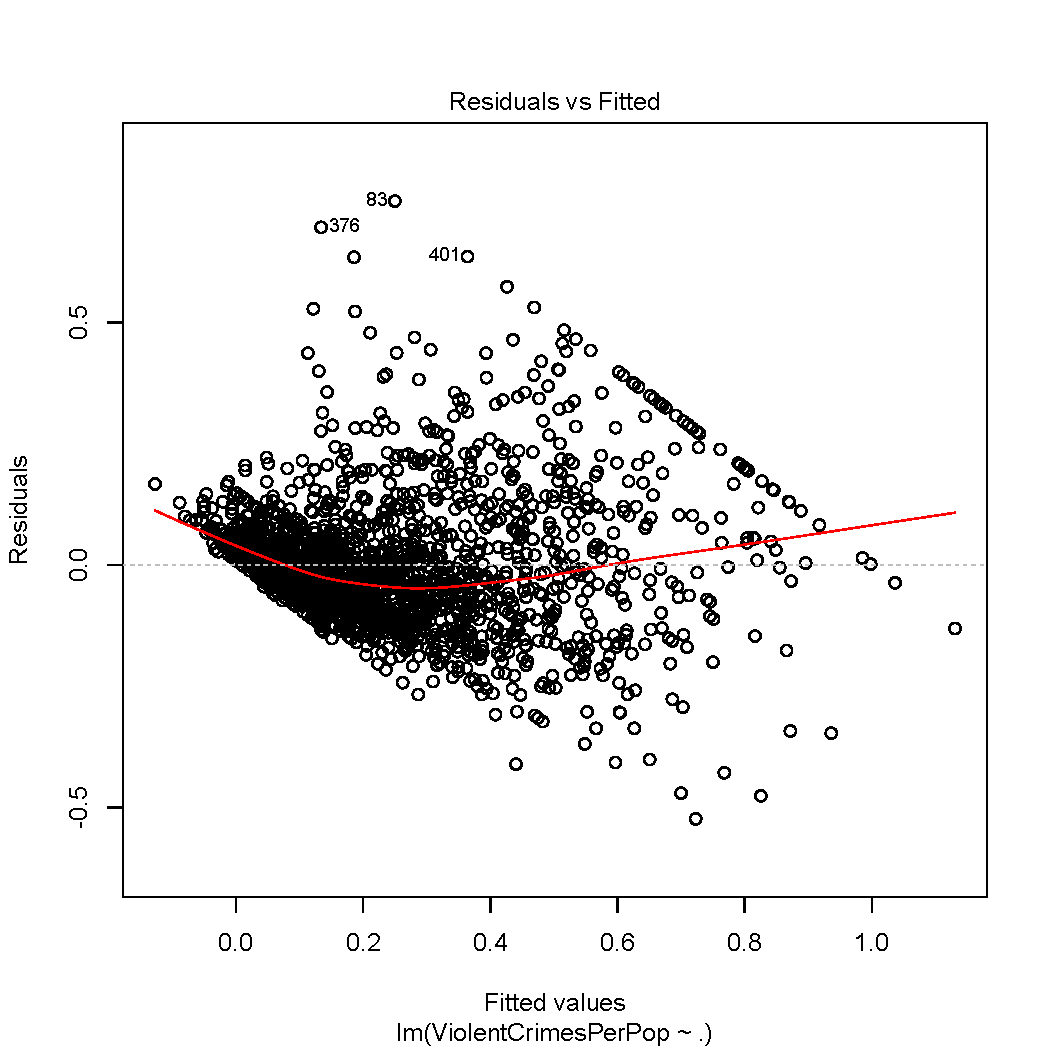
\includegraphics[width=0.7\textwidth,trim= 0 0 20 30, clip]{Linear_regression_residuals.pdf}
\end{figure}

\vspace{-0.5cm}
\begin{figure}[h!]
    \centering
    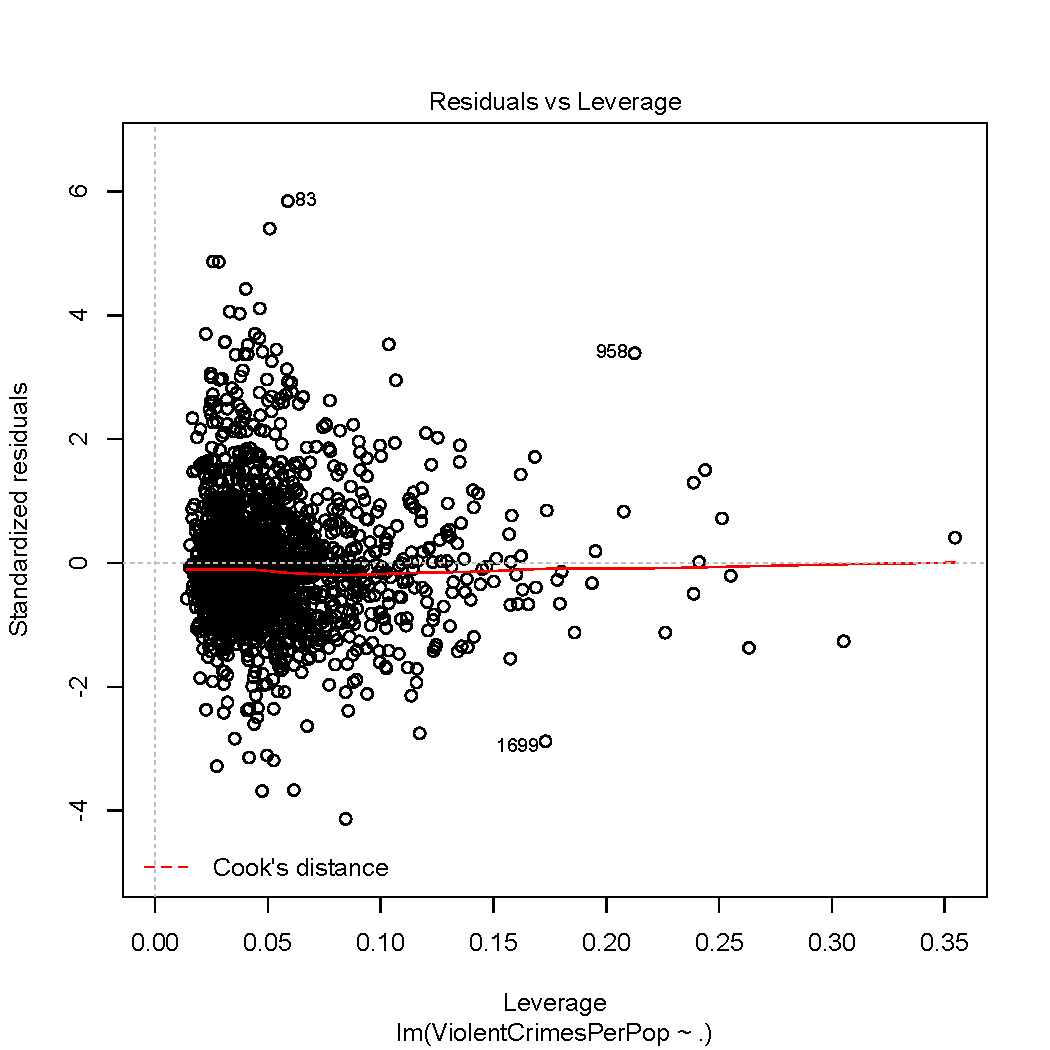
\includegraphics[width=0.7\textwidth,trim= 0 0 20 30, clip]{Linear_regression_cook.pdf}
\end{figure}
\FloatBarrier

\newpage
\subsubsection{Box-Cox transformed data}
\vspace{-0.5cm}
\begin{figure}[h!]
    \centering
    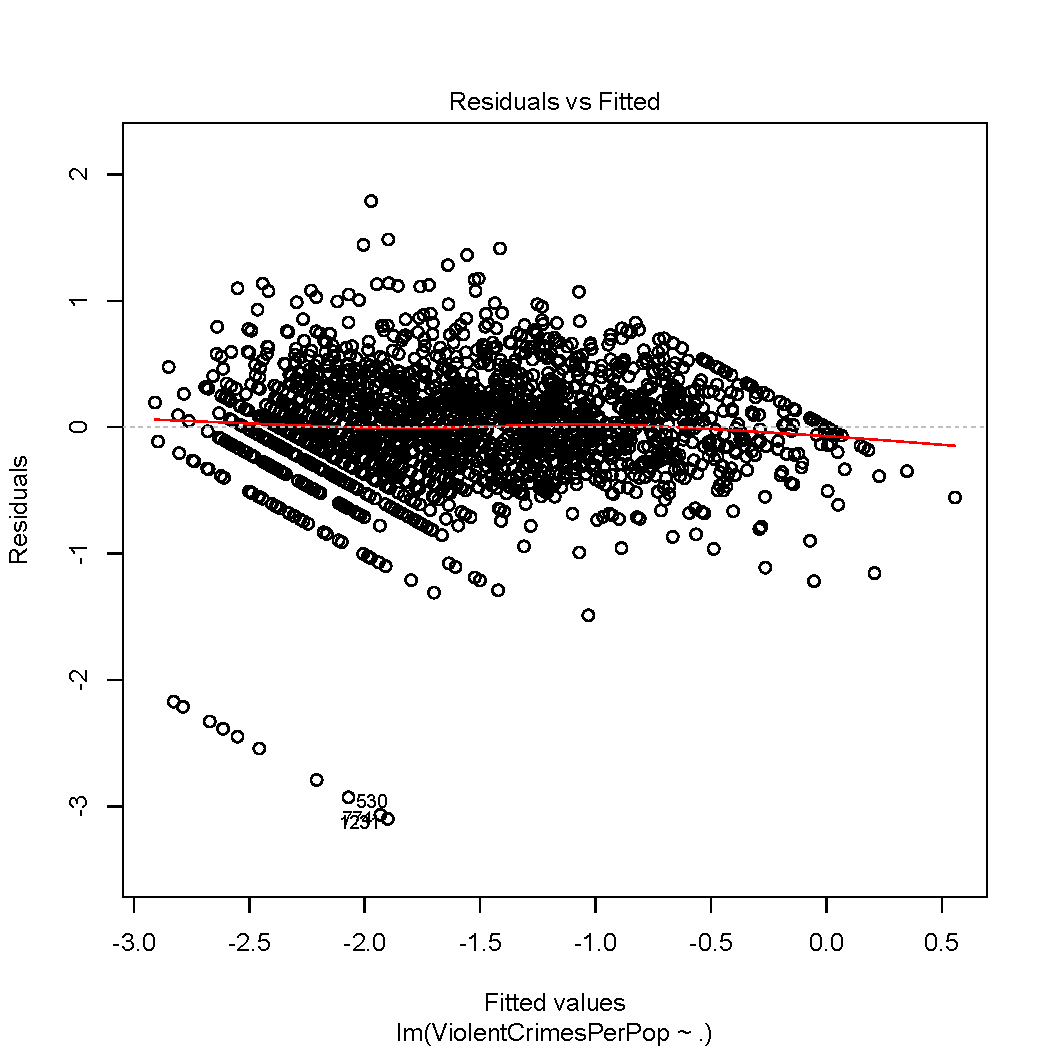
\includegraphics[width=0.7\textwidth,trim= 0 0 20 30, clip]{Boxcox_regression_residuals.pdf}
\end{figure}
\FloatBarrier

\vspace{-0.5cm}
\begin{figure}[h!]
    \centering
    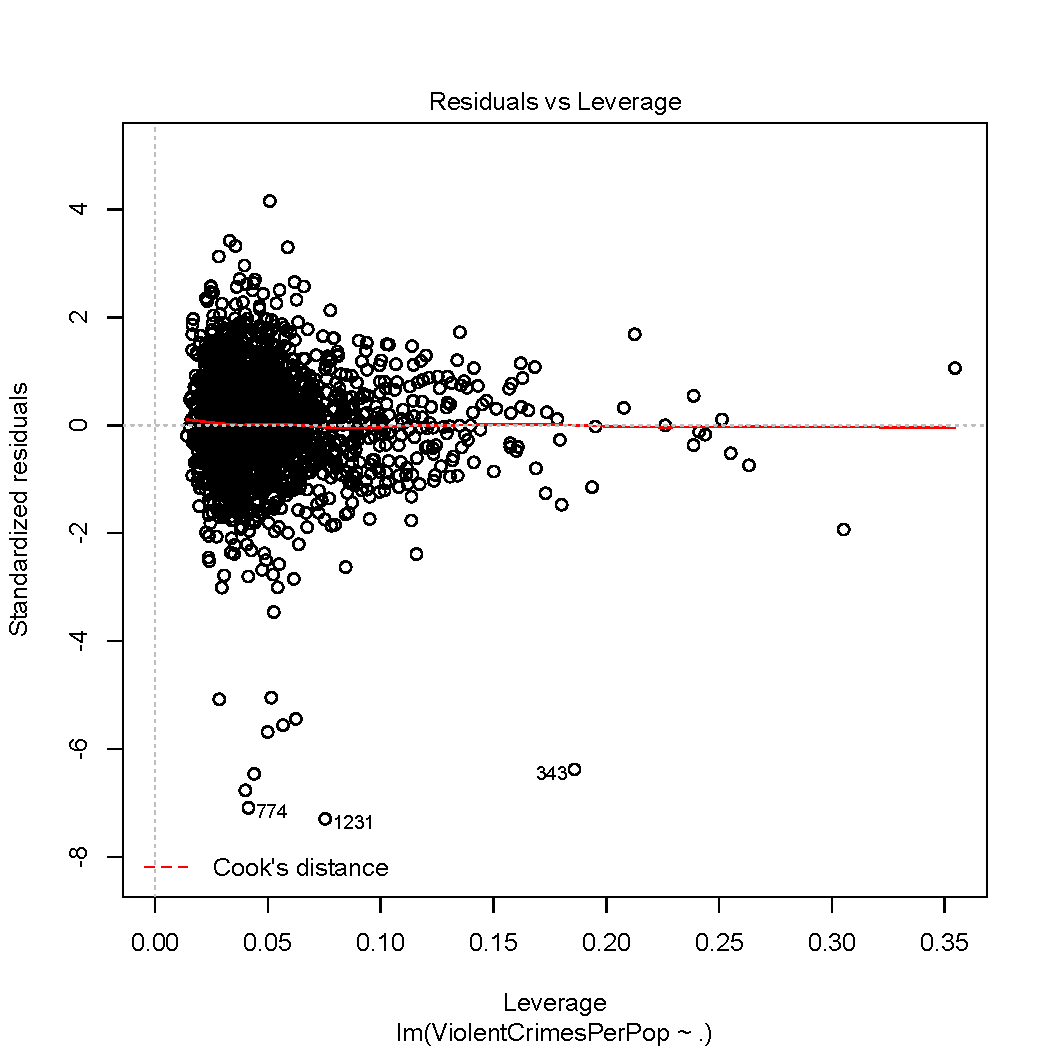
\includegraphics[width=0.7\textwidth,trim= 0 0 20 30, clip]{Boxcox_regression_cook.pdf}
\end{figure}
\FloatBarrier

\subsection{Conclusions}
\subsubsection{Standard data}
The Mean-squared error on both the full regression 
and the tested regression are both quite small. 
The tested regression Mean-squared error is a little larger as it has less data

The residual graph was relatively poorly behaved with some strange linear structures.
The lack a ``banna'' shows that our problem is not likely to be fixed by Boxcox or other types of transformed. We need more explanatory values.
According to the Residuals VS Leverage graph no points had undue influence
or worry some cooks distance.

This show that the regression is likely possible with our data but needs work.


\subsubsection{Box-Cox transformed data}
Our Boxcox transformed data looked promising but has a larger Mean-squared error.
The residual graph shows that while the data looks straighter the linear structures can still be seen.
However the when one accounts for the change in base in the distortion graph looks far worse. We also see that at low fitted values the data looks split and some have extremely low Residuals. This is likely caused by values extremely close to zero.

Boxcox was useless. 

\section{Basics - Nearest Neighbor regression}
\subsection{Implementation}
\lstinputlisting[firstline=84, lastline=112]{crimes.R}

\subsection{Results}

- Mean-squared error on the test data (20\%): 3.64e-02


\vspace{-0.5cm}
\begin{figure}[h!]
    \centering
    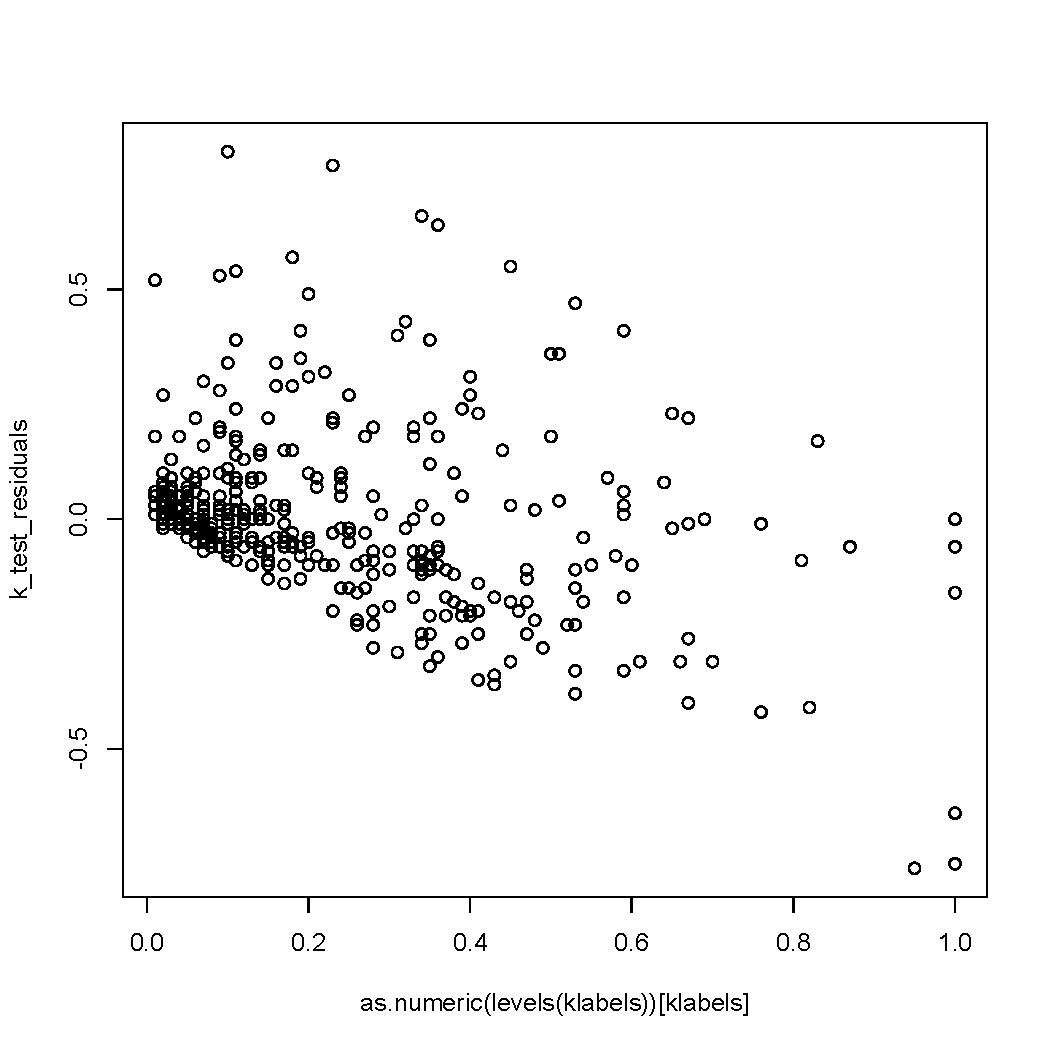
\includegraphics[width=0.7\textwidth,trim= 0 0 20 30, clip]{NN_regression_residuals.pdf}
\end{figure}
\FloatBarrier


\subsection{Conclusions}
The Mean-squared error on k-nearest neighbor regression did not work as well as the
 linear regression. It's  Mean-squared error was signifantly higher and looks worse.
 Scaling the data changed nothing. I am guessing that the data set was prescaled.

\section{Dealing with missing values}
\subsection{Implementation}

\lstinputlisting[firstline=114, lastline=163]{crimes.R}


\subsection{Results}
Linear Regression (imputed missing values):
 - Mean-squared error on the test data (20\%): 1.88e-02
Nearest Neighbours (imputed missing values):
 - Mean-squared error on the test data (20\%): 1.00e-01

\newpage
\subsubsection{Linear regression}
\vspace{-0.5cm}
\begin{figure}[h!]
    \centering
    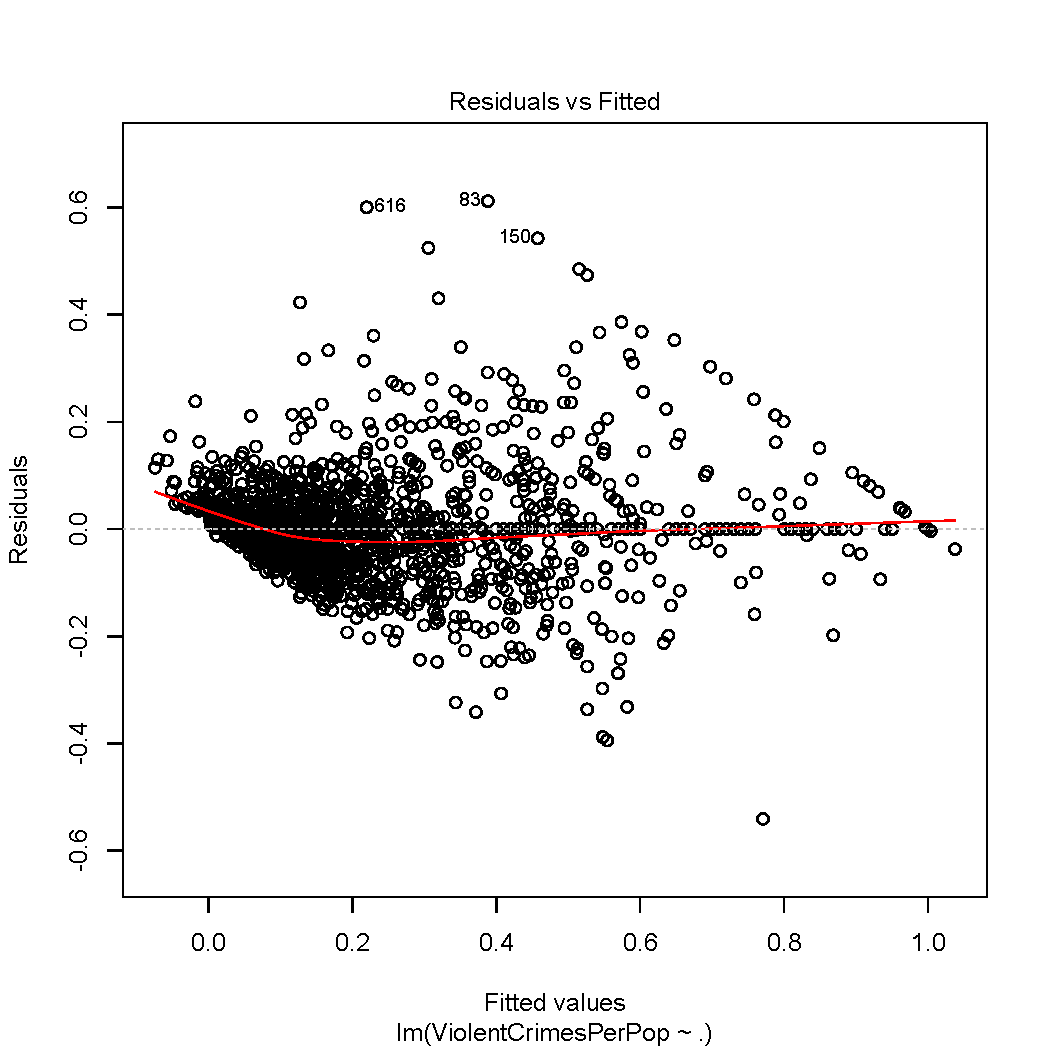
\includegraphics[width=0.7\textwidth,trim= 0 0 20 30, clip]{Unk_linear_regression_residuals.pdf}
\end{figure}
\FloatBarrier

\vspace{-0.5cm}
\begin{figure}[h!]
    \centering
    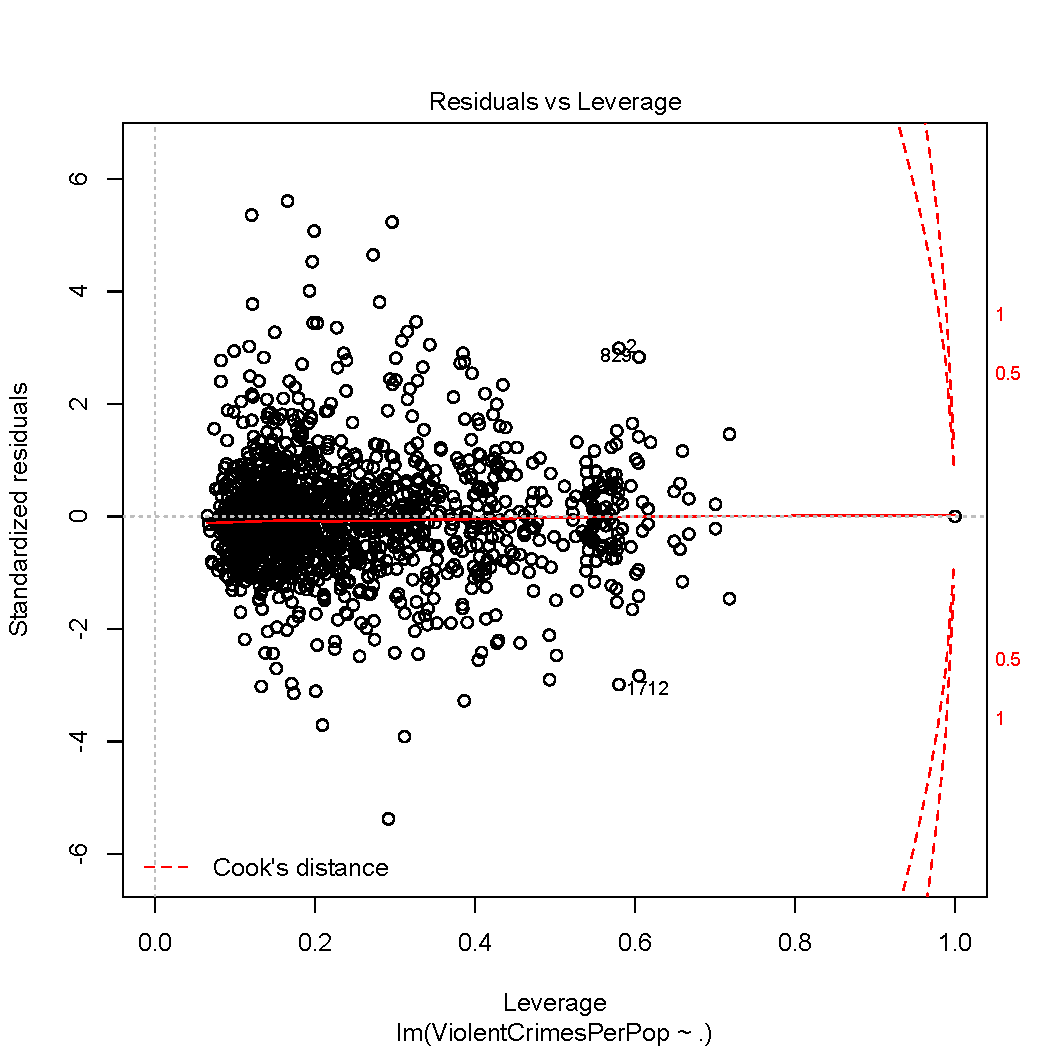
\includegraphics[width=0.7\textwidth,trim= 0 0 20 30, clip]{Unk_linear_regression_cook.pdf}
\end{figure}
\FloatBarrier

\newpage
\subsubsection{Nearest Neighbours}
\vspace{-0.5cm}
\begin{figure}[h!]
    \centering
    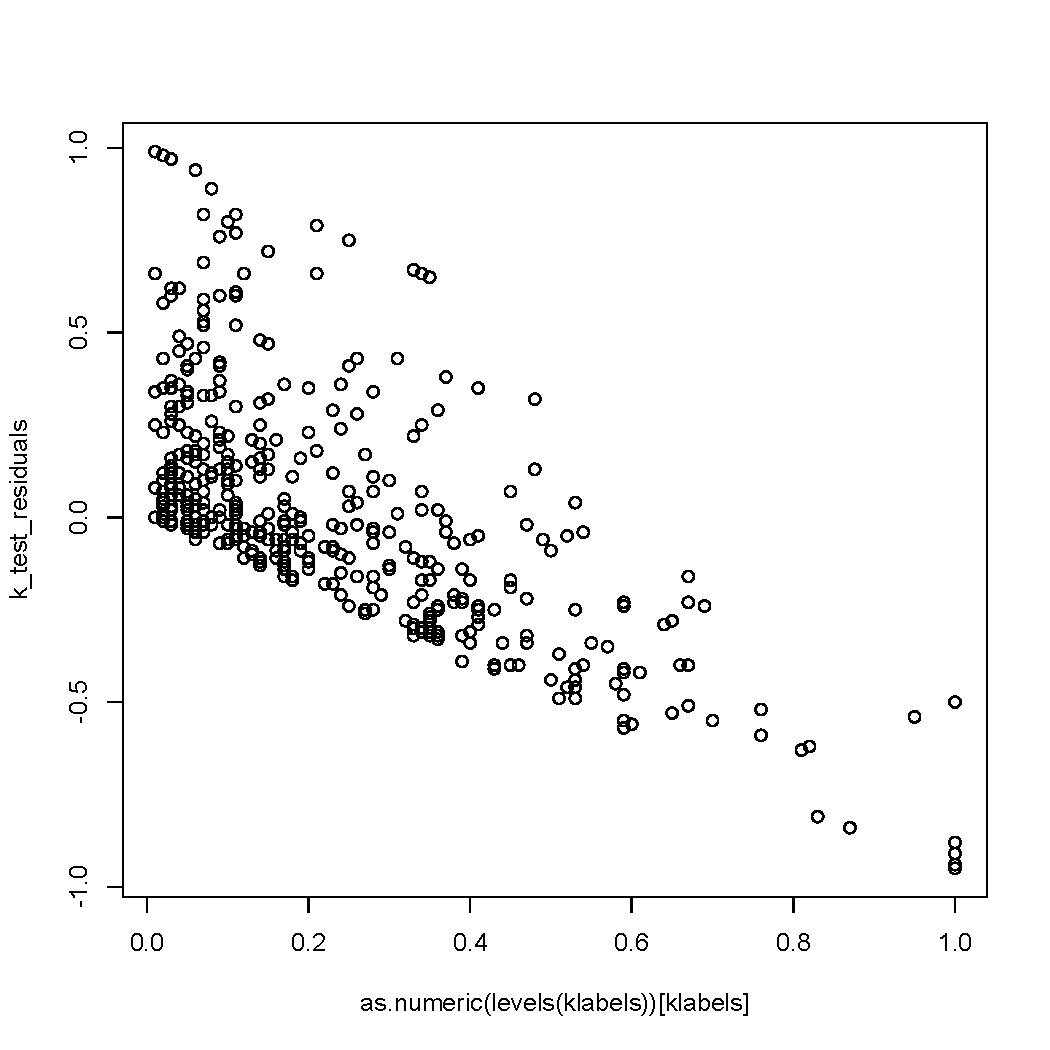
\includegraphics[width=0.7\textwidth,trim= 0 0 20 30, clip]{Unk_NN_regression_residuals.pdf}
\end{figure}
\FloatBarrier

\subsection{Conclusions}

\section{Modified Nearest Neighbours}
\subsection{Implementation}
\lstinputlisting{nn-modified.R}

\vspace{-0.4cm}
\subsection{Conclusions}
Two different implementations have been tried for this exercise, one that computes the distance between two vectors with some question mark elements in a linear way (\texttt{distance\_lin}) and other that does the same but with vectorial operations (\texttt{distance\_vec}). \\

Unfortunately, the linear code that uses this distance functions and other \texttt{R} specific instructions to apply the function to matrix columns, like \texttt{outer}, were so slow during the execution that it was impossible to obtain results.

\end{singlespace}
\end{document}
